\documentclass[12pt,a4paper]{report}

%------------------------------------------------------------------------
% PACKAGES:

\usepackage{lmtstyle}
% Define typearea
% a) Use automatic:
\usepackage[BCOR1cm]{typearea}
% b) Or use fixed:
%\usepackage{geometry}
%\geometry{left=1.5cm,textwidth=18.5cm,top=1.5cm,textheight=26.5cm}
\usepackage[american,ngerman]{babel}
% Use list of tabels, etc. in table of contents:
\usepackage{tocbibind}
% German paragraph skip
\usepackage{parskip}
% Encoder:????
\usepackage[latin1]{inputenc}
%\usepackage[applemac]{inputenc}
% Use A4-paper efficiently:
\usepackage{a4wide}
% Index-generation
\usepackage{makeidx}
% Einbinden von URLs:
\usepackage{url}
% Include .eps-files (needed also for the TUM-logo):
%\usepackage{epsf}
% Special \LaTex symbols (e.g. \BibTeX):
\usepackage{doc}
% Include Graphic-files:
%\usepackage{graphics}
% Include Graphic-files:
\usepackage{graphicx}
% Include doc++ generated tex-files:
%\usepackage{docxx}
% Include PDF links
%\usepackage[pdftex, bookmarks=true]{hyperref}
%------------------------------------------------------------------------
\usepackage{amsmath,amsfonts,amssymb,amsthm}
\usepackage{mathtools}
\usepackage{commath}
\usepackage[sc,osf]{mathpazo}
\usepackage{subcaption}
\usepackage{amsmath}
\usepackage{float}
\usepackage{listings}
\usepackage{xcolor}

\lstset{language=C++,
numbers=left,
                basicstyle=\ttfamily,
                keywordstyle=\color{blue}\ttfamily,
                stringstyle=\color{red}\ttfamily,
                commentstyle=\color{green}\ttfamily,
                morecomment=[l][\color{magenta}]{\#}
}

\graphicspath{{figures/}}

\newcommand{\inlinecode}[2]{\colorbox{white}{\lstinline[language=#1]$#2$}}

%########################################################################
% CHOOSE DEFAULT LANGUAGE:
%\setlang{de}
\setlang{en}

% FILL IN ACCORDINGLY:
\title{Parallel mesh simplification}
\type{Interdisciplinary project (IDP)}
\author{Zielonka Wojciech}
\matrikelnr{03704591}
\street{Am Sch�feranger 15}
\town{85764 Oberschlei�heim}
\advisor{Prof. Dr.-Ing. Eckehard Steinbach}
\datebegin{01.04.2019}
\dateend{01.11.2019}
%########################################################################


\begin{document}%****************************************************

\makemtgtitle

% MAIN PART:
\pagenumbering{roman}
% German abstract:
\switchlanguage{de} % The Kurzfassung, if given, is supposed to be in German!

\thispagestyle{plain}

\section*{Kurzfassung} 
In der Kurzfassung werden auf einer halben Seite das Problemfeld und
die pr�sentierten Ergebnisse zusammengefasst.

\switchlanguage{\lang} % Switch back to the docmuent's default language.
% English abstract:
\switchlanguage{en} % The abstract is supposed to be in English!

\thispagestyle{plain}

\section*{Abstract}
This work elaborates a new parallel algorithm based on quadric error metric and adaptive thresholding to simplify a triangle mesh. The approach emphasizes planar surfaces as a target to simplify. The main goal was to create a framework able to produce high quality progressive meshes for browser streaming purposes.

\switchlanguage{\lang} % Switch back to the document's default language.

% Table of contents:
\tableofcontents 

% Introduction (Einleitung):
\chapter{Introduction}
\pagenumbering{arabic}%Ab hier, werden arabische Zahlen benutzt
\setcounter{page}{1}%Mit Abschnitt 1 beginnt die Seitennummerierung neu.
\thispagestyle{empty}

Mesh simplification is necessary when one wants to reduce the size of a mesh while still preserving geometry. The technique is widely used in computer graphics to change the model level of details \cite{lod03}. This project elaborates a specific case of mesh simplification, where the focus is mostly on planar surfaces, like walls and floors, at the same time, keeping high level of details for complex shapes; plants, elements on desks in an office, etc. Mesh reconstruction in general introduces a problem of using the same level of details for the whole $3D$ space. Most of planar surfaces can be described with reduced amount of triangles. Therefore, after generating a reconstructed mesh from real-world environments, mapped by static or mobile scanners, we can successfully apply simplification with great results. In the next chapter, I will elaborate foundations for the geometric error metric. Forwarded by the introduction to the extended version of this algorithm, which additionally uses color and normals for the error metric. Finally, in the forth chapter, I will describe the parallel approach with adaptive thresholding to solve the problem.

% Text Body (Hauptteil)
% Could have multiple chaper-files, e.g.:
\chapter{Basic Simplification Algorithm}
\thispagestyle{empty}% no page number in chapter title page
In this section I will present a basic algorithm for mesh simplification which is founded on serverl fundamental components: iterative vertex contraction, quadric error metric, mesh clustering and parallel strategy to consume those clusters. In this chapter I will elaborate each of those parts considering surface geometry alone. In the next chapter I will introduce the extended version of this algorithm which additionaly uses color and normals for the error metric.
\numberwithin{equation}{section}
\section{Design}
The core of the algorithm is based on Michael Garland's work Quadric-Based Polygonal Surface Simplification \cite{garland99} where he suggests an algorithm capable of producing high-quality approximations of polygonal meshes. The main assumption is that the approximation need not to maintain the topology of the original surface and is a nicely balanced trade of between quality and size. 

The goal of this work was to adopt this algorithm to a parallel framework capable of fast progresive mesh streaming [citation] for renderer engines in browsers. An example of such a renderer is Indoorviewer product created by NavVis. Depending on selected mesh resolution and level of details an appropriate mesh will be streamed to a browser. Therefore, the size and quality is crucial for the endpoint users to get maximal usability. Using the assumption that planar surfaces need much less trinagles to describe geometry we can get light and detailed meshes which are perfect for streaming purposes.
\clearpage

\section{Iterative Vertex Contraction}
The simplification algorithm is based on several atomic operations. The most important of them is an edge contraction. Let me denote an edge as a pair of vertices $(\mathbf{v_i}, \mathbf{v_j})\rightarrow\bar{\mathbf{v}}$. The atomic opartion of a contraction is then defined as:

\begin{enumerate}
\item Move the vertices $\mathbf{v_i}$ and $\mathbf{v_j}$ to the position $\bar{\mathbf{v}}$
\item Replace all connections of $\mathbf{v_j}$ with $\mathbf{v_i}$
\item Remove $\mathbf{v_j}$ and all faces which belong both to $\mathbf{v_i}$ and $\mathbf{v_j}$. In Figure~\ref{fig:edge_contraction_ref} the gray faces.
\end{enumerate}

\begin{figure}[h!]
  \begin{center}
    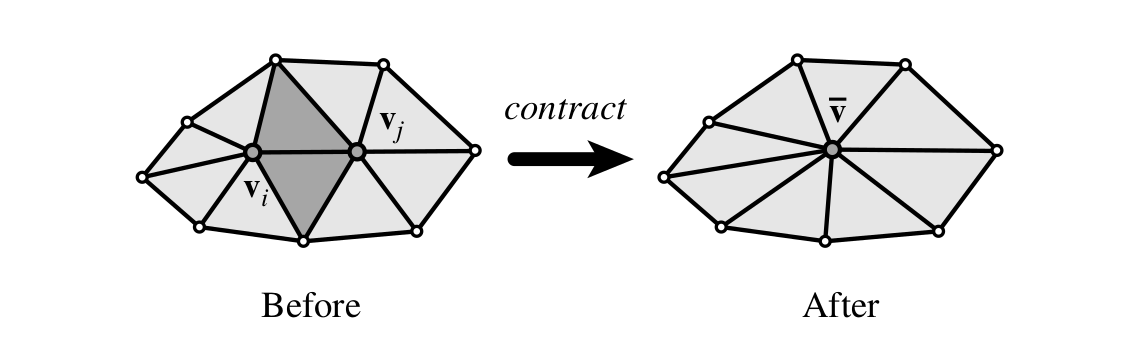
\includegraphics[width=17cm]{edge_contraction}
    \caption{Contraction of an edge \cite{garland99}.}
    \label{fig:edge_contraction_ref}
  \end{center}
\end{figure}

In the parallel framework the crucial aspect is locking all vertices and faces for the current edge to prevent from multiple threads modify the same region. To achieve this, $tryLock()$ method was used. To perform a contraction we have to check if it is possible to lock the whole neighbourhood, in the other case, it means that already a different thread is manipulating a given region. In such a situation the contraction is stopped.

The algorithm is a greedy procedure \cite{cormen01} driven by the cost of contraction. To achieve simplification we apply a sequence of edge contraction. Where the sequence is created as follows \cite{garland97}:

\begin{enumerate}
\item Select a set of candidate vertex pairs.
\item Assign a cost of contraction to each candidate.
\item Place all candidates in a heap keyed on cost with the minimum cost pair at the top.
\item Repeat until the desired approximation is reached:
\begin{enumerate}
\item Remove the pair $(\mathbf{v_i}, \mathbf{v_j})$ of least cost from the heap.
\item Contract this pair.
\item Update costs of all candidate pairs involving $\mathbf{v_i}$.
\end{enumerate}
\end{enumerate}

Each edge is associated with a cost of contraction which is basically the amount of error made during deletion of a given pair of vertices.  This cost is a key in the minimum heap \cite{cormen01} which is iteratively $pop()$. In each main iteration (steps from 1 to 4) we contract edges up to the current adaptive threshold level. If a current edge's cost is bigger or equal than the acceptable error, the main iteration procedure is stopped and the remaining egdes in the heap are ignored. In a next iteration the error is slightly increased in such a way that perviously contracted regions are even more simplified. The error calculations are based on a hyperparameter $aggressiveness$ and a current iteration value:
\begin{align}
error(i)=0.000000001*(i+3)^a
\end{align}
where $i$ is the iteration and $a$ is the aggressiveness.

\section{Assessing Cost of Contraction}
In this section I will elaborate how to measure the cost of contraction of an edge just for geometry attributes. Maintaining high level of details and faithful representation of original we should reflect the cost in the effect of changing the surface. Meaning, if the error is small the geometry changes insignificantly. An edge with a small error is a perfect candiate for removal.

Because the metric is plane-based, first, let me define a standard representation of a plane as $\mathbf{n}^T\mathbf{v}+d=0$ where $\mathbf{n} = [a\;b\;c]^T$, $d$ is a scalar constant and $\mathbf{v} = [x\;y\;z]^T$. From this, we can formulate quadric error metric as following \cite{garland99}:
\begin{align}
D^2(\mathbf{v}) = (\mathbf{n}^T\mathbf{v}+d)^2 = (ax + by + cz + d)^2
\label{quadric_distance}
\end{align}
The error for the set of planes associated with the vertex $v$ is then defiend as:
\begin{align}
\sum_{i} D_i^2(\mathbf{v}) = \sum_{i} (\mathbf{n_i}^T\mathbf{v}+d_i)^2
\end{align}
Each vertex has accumulated error metric value for surrounding faces  which represents maximum squared distance to the intersection of all planes spanned by each face.

Figure~\ref{fig:measuring_contraction_ref} shows how finding an optimal point $\bar{v}$ could look in practice in 2D. Vertices $v_i, v_j$ define set of planes $P_i = \{A,C\}$ and $P_j = \{B, C\}$. The error on each of those vertices equals $E_{plane}(v_i) = E_{plane}(v_j) = 0$ since they both lie on the lines span by thier sets. Let me define a new set which is a union of $ \bar{P} = P_i \cup P_j = \{ A,B,C \}$. Position of $\bar{v}$ minimizes the sum of square distances the the lines in $\bar{P}$ \cite{garland99}.

\begin{figure}[H]
  \begin{center}
    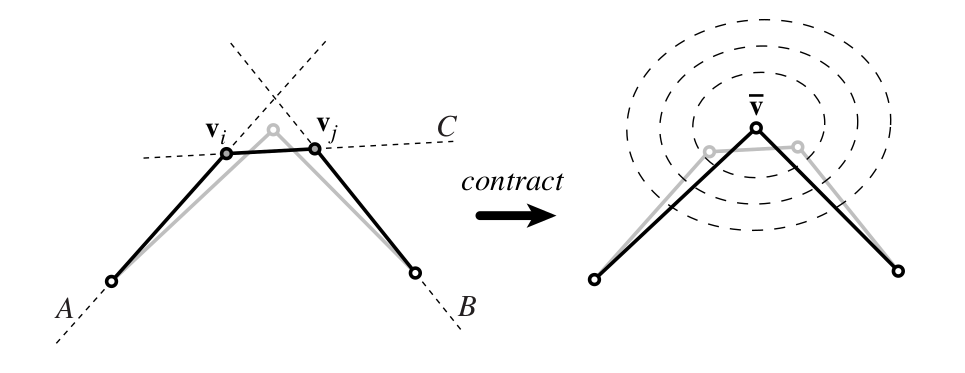
\includegraphics[width=15cm]{measuring_contraction}
    \caption{Measuring contraction cost in 2D \cite{garland99}.}
    \label{fig:measuring_contraction_ref}
  \end{center}
\end{figure}

\section{Quadric Error Metric}

In this section I will introduce the compact representation of the quadric error. First, let me expand the previously declared quadric distance $D^2(\mathbf{v})$~\ref{quadric_distance}.
\begin{align}
D^2(\mathbf{v})&=(\mathbf{n}^T\mathbf{v}+d)^2\\
	  &=(\mathbf{n}^T\mathbf{v}+d)(\mathbf{n}^T\mathbf{v}+d)\\
	  &=(\mathbf{v}^T\mathbf{n}\mathbf{n}^T\mathbf{v}+2d\mathbf{n}^T\mathbf{v}+d^2)\\
	  &=(\mathbf{v}^T(\mathbf{n}\mathbf{n}^T)\mathbf{v}+2(d\mathbf{n})^T\mathbf{v}+d^2)
	  \label{quadric_equation}
\end{align}
where $\mathbf{n}\mathbf{n}^T$ is the outer prodcut of
\begin{align}
\left[
\begin{array}{rrrr}
a^2 & ab & ac   \\
ab  & b^2 & bc  \\
ac  & bc  & c^2 \\
\end{array}\right]
\end{align}
Therefore, the $quadric\;Q$ is defined as a tripe:
\begin{align}
Q = (\mathbf{A},\mathbf{b},c)
\end{align}
Where $\mathbf{A}$ is a $3x3$ matrix, $\mathbf{b}$ is a 3-vector and c is a scalar. We can now rewrite the~\ref{quadric_equation} equation to:
\begin{align}
Q(\mathbf{v}) = \mathbf{v}^T\mathbf{A}\mathbf{v} + 2\mathbf{b}^T\mathbf{v} + c
\end{align}
Quadrics provide an intuitive addition operation which is component-wise: $Q_i(\mathbf{v}) + Q_j(\mathbf{v}) = (Q_i + Q_j)(\mathbf{v})$ where $Q_i(\mathbf{v}) + Q_j(\mathbf{v}) = (\mathbf{A_i} + \mathbf{A_j}, \mathbf{b_i} + \mathbf{b_j}, c_i + c_j)$. Using this fact we can easily define a single quadric $E_Q$ for the set of planes of a given vertex \cite{garland99} as sum over qudrics for each face:
\begin{align}
E_Q(\mathbf{v}) = \sum_{i} D_i^2(\mathbf{v}) = \sum_{i} Q_i(\mathbf{v}) = Q(\mathbf{v})
\end{align}
In other words, each vertex contains accumulated information about the error for the whole local neighbourhood of $\mathbf{v}$. For the pair of vertices the cost of contraction $(\mathbf{v_i}, \mathbf{v_j})\rightarrow\bar{\mathbf{v}}$ is simply:
\begin{align}
Q(\mathbf{\bar{v}}) = Q_i(\mathbf{\bar{v}}) + Q_j(\mathbf{\bar{v}})
\end{align}
The value of $Q(\mathbf{\bar{v}})$ is a key in the min-heap. Tables~\ref{tab:approx_bunny_ref} and~\ref{tab:wireframe_ref} show an example of simplification using quadric metric. Due to complexity of the original Stanford Bunny mesh which has 69451 faces, I first simplified it to 3642 faces and used this as a reference model.

\begin{table}[h!]
\centering
\begin{tabular}{ |c|c| } 
 \hline
 Number of faces & Original simplification\\
 \hline
 3642 faces & 94.756 \\ 
 2228 faces & 96.791 \\ 
 1842 faces & 97.347\\ 
 1152 faces & 98.341\\ 
 665 faces & 99.042\\ 
 130 faces & 99.813\\
 \hline
\end{tabular}
\caption{Percentage of simplification of the original Stanford Bunny with 69351 faces.}
\end{table}
Table~\ref{tab:original_ref} shows the quality of progressive simplification. As you can see, 70\% of reduction is hard to distinguish from the original mesh, even the 94\% is still a good approximation and features of the bunny are preserved fairly well.

\begin{center}
  	\begin{table}[H]
  	\begin{center}
  	\begin{tabular}{cc}
	\begin{subfigure}{0.7\textwidth}\centering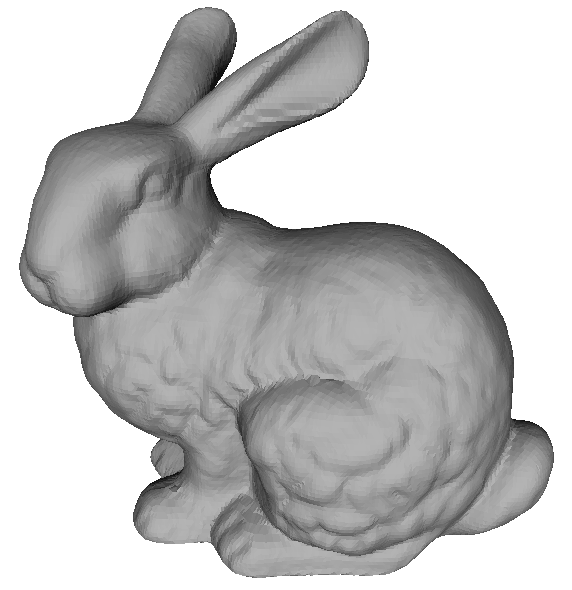
\includegraphics
		[width=0.5\columnwidth]{original_100}\caption{Faces 69451 (100\%)}\label{original_100_ref}\end{subfigure}\\
	\begin{subfigure}{0.7\textwidth}\centering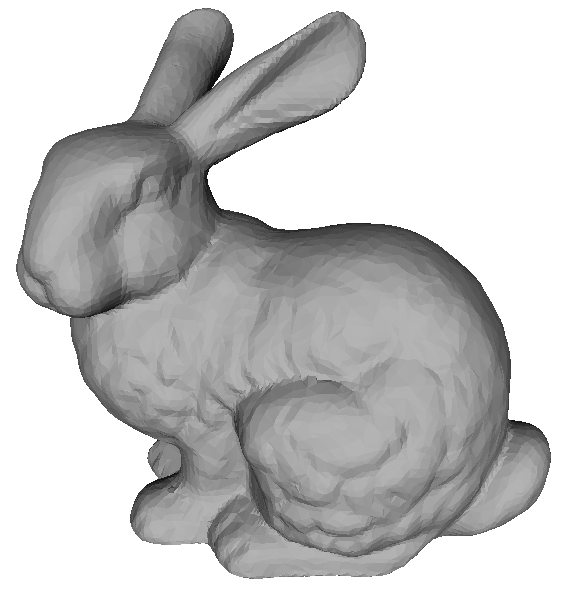
\includegraphics
		[width=0.5\columnwidth]{original_70}\caption{Faces 18892 (30\%)}\label{original_70_ref}\end{subfigure}\\
	\begin{subfigure}{0.7\textwidth}\centering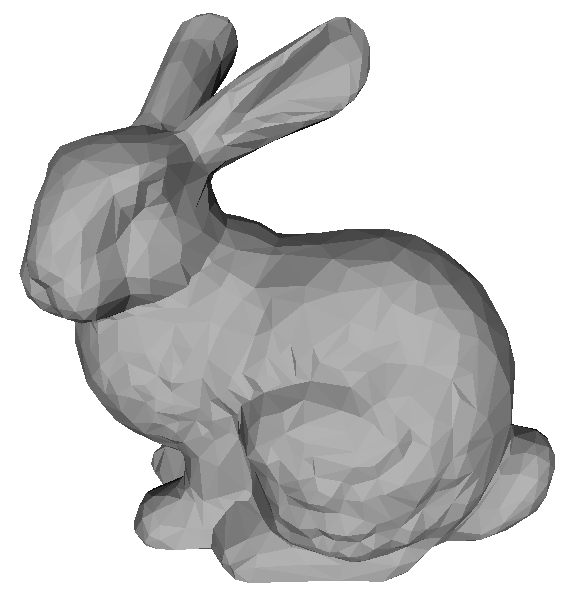
\includegraphics
		[width=0.5\columnwidth]{original_95}\caption{Faces 3642 (6\%)}\label{original_95_ref}\end{subfigure}\\
	\end{tabular}
	\caption{Quality of the simplification of the original mesh.}
  	\label{tab:original_ref}
  	\end{center}
	\end{table}
\end{center}

\begin{center}
  	\begin{table}[H]
  	\begin{center}
  	\begin{tabular}{cc}
	\begin{subfigure}{0.4\textwidth}\centering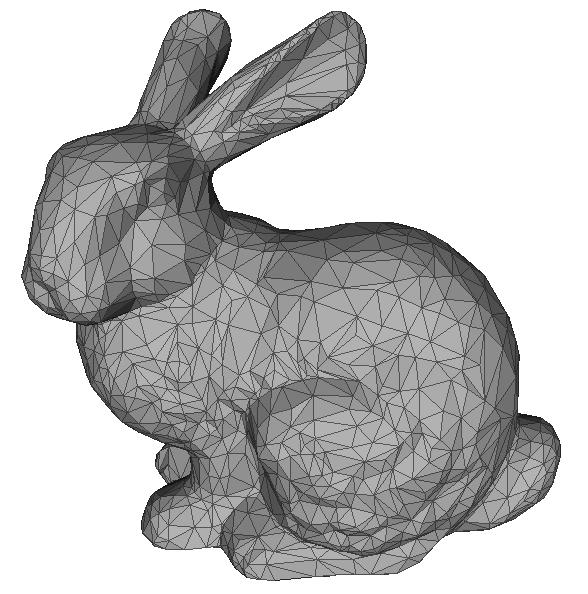
\includegraphics
		[width=0.7\columnwidth]{bunny_100}\caption{Faces 3642}\label{ref_label1}\end{subfigure}&	
	\begin{subfigure}{0.4\textwidth}\centering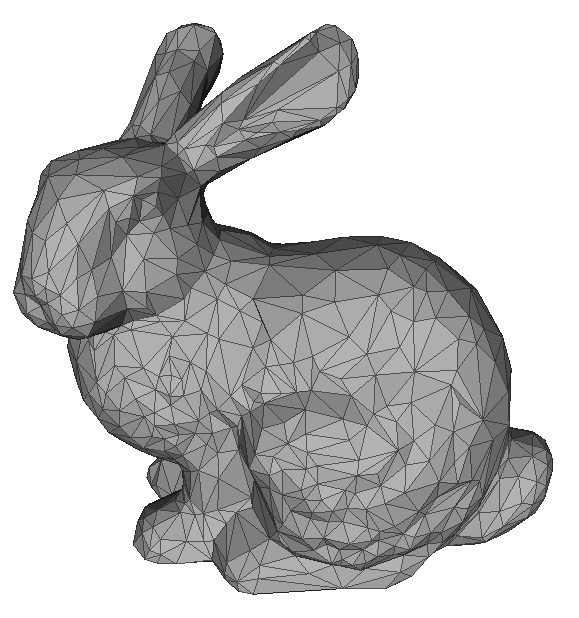
\includegraphics
		[width=0.7\columnwidth]{bunny_80}\caption{Faces 2228}\label{bunny_80_ref}\end{subfigure}\\
	\newline
	\begin{subfigure}{0.4\textwidth}\centering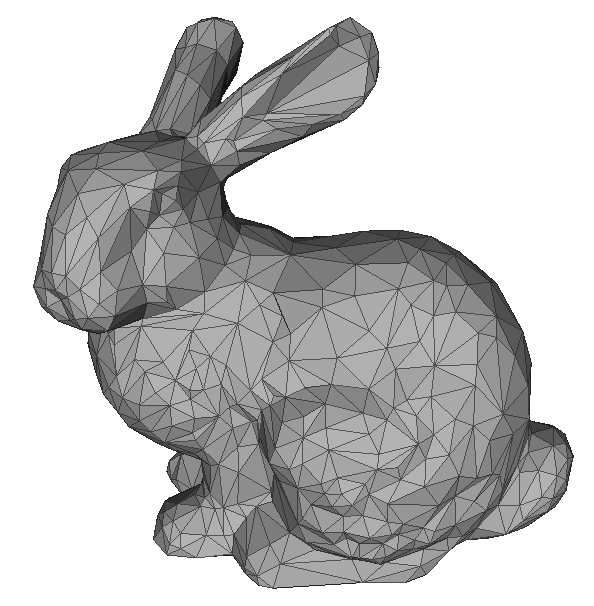
\includegraphics
		[width=0.7\columnwidth]{bunny_70}\caption{Faces 1842}\label{bunny_70_ref}\end{subfigure}&
	\begin{subfigure}{0.4\textwidth}\centering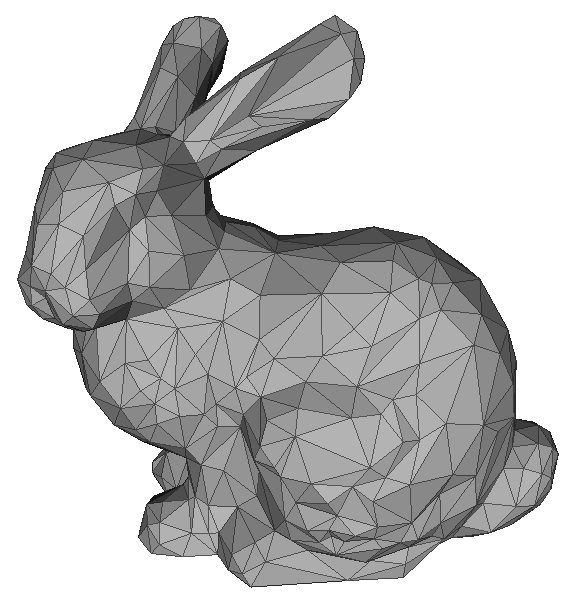
\includegraphics
		[width=0.7\columnwidth]{bunny_60}\caption{Faces 1152}\label{bunny_60_ref}\end{subfigure}\\
	\newline
	\begin{subfigure}{0.4\textwidth}\centering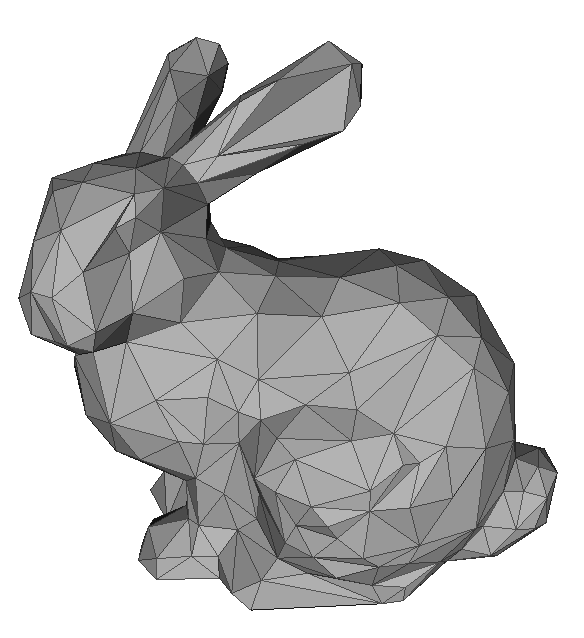
\includegraphics
		[width=0.7\columnwidth]{bunny_50}\caption{Faces 655}\label{bunny_50_ref}\end{subfigure}&
	\begin{subfigure}{0.4\textwidth}\centering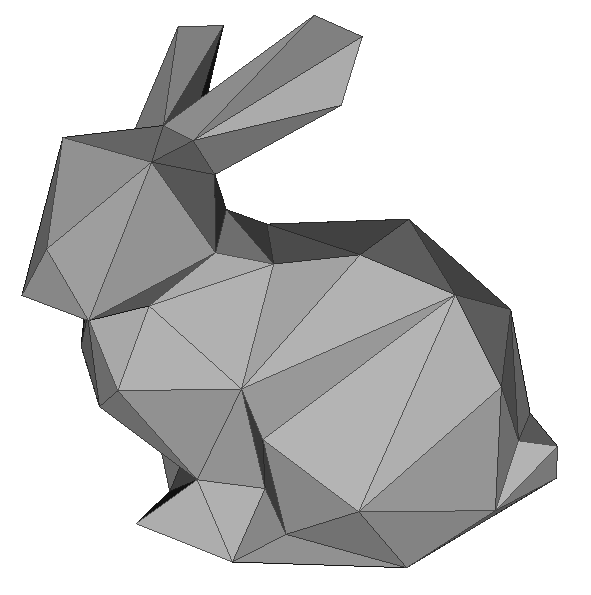
\includegraphics
		[width=0.7\columnwidth]{bunny_40}\caption{Faces 130}\label{bunny_40_ref}\end{subfigure}\\
	\end{tabular}
  	\caption{Several approximations of Stanford Bunny constructed with the geometry quadric error metric.} \label{tab:approx_bunny_ref}
  	\end{center}
	\end{table}
\end{center}

\begin{center}
  	\begin{table}[H]
  	\begin{center}
  	\begin{tabular}{cc}
	\begin{subfigure}{0.4\textwidth}\centering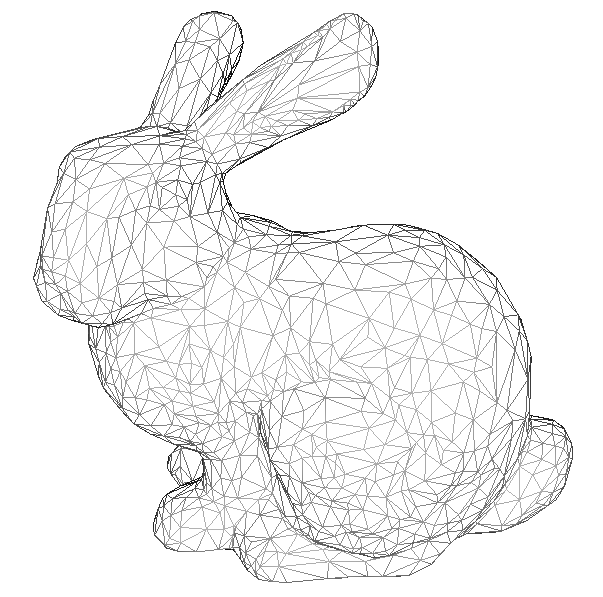
\includegraphics
		[width=0.7\columnwidth]{wireframe_100}\caption{Faces 3642}\label{wireframe_100_ref}\end{subfigure}&	
	\begin{subfigure}{0.4\textwidth}\centering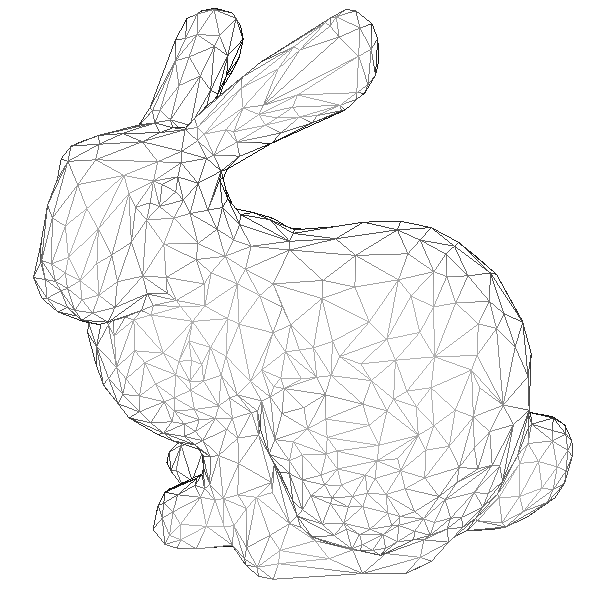
\includegraphics
		[width=0.7\columnwidth]{wireframe_80}\caption{Faces 2228}\label{wireframe_80_ref}\end{subfigure}\\
	\newline
	\begin{subfigure}{0.4\textwidth}\centering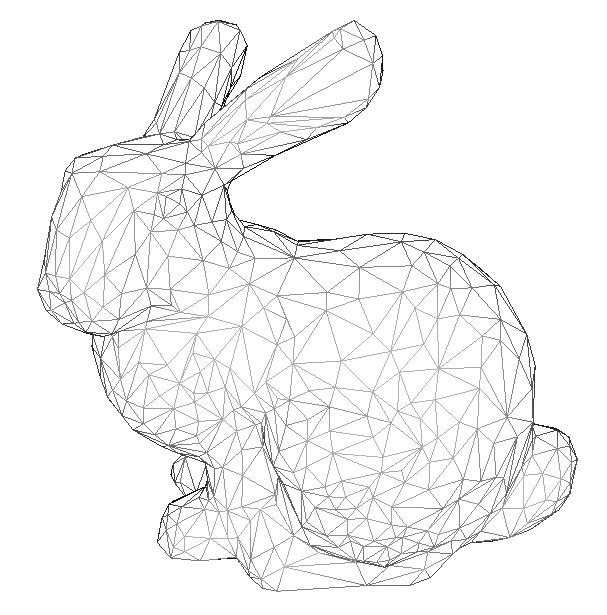
\includegraphics
		[width=0.7\columnwidth]{wireframe_70}\caption{Faces 1842}\label{wireframe_70_ref}\end{subfigure}&
	\begin{subfigure}{0.4\textwidth}\centering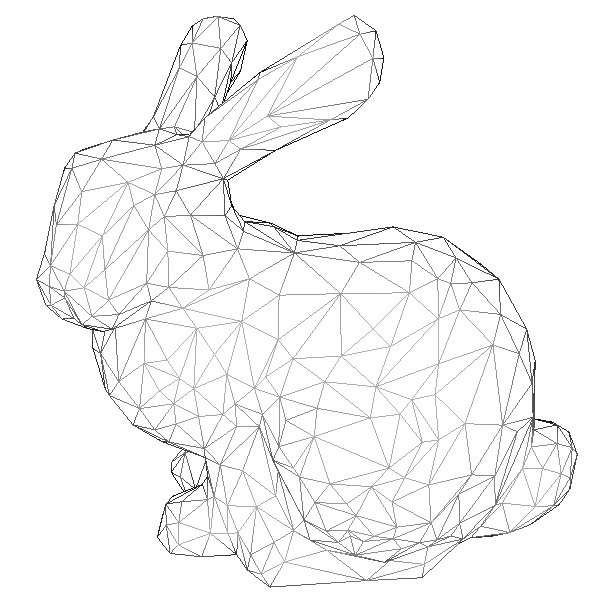
\includegraphics
		[width=0.7\columnwidth]{wireframe_60}\caption{Faces 1152}\label{wireframe_60_ref}\end{subfigure}\\
	\newline
	\begin{subfigure}{0.4\textwidth}\centering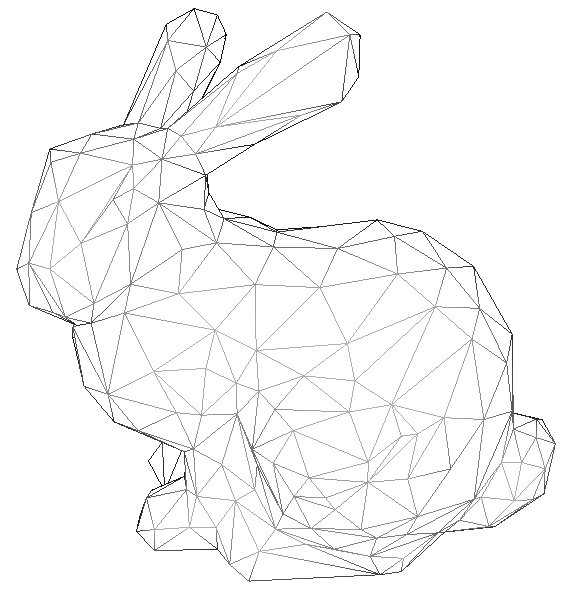
\includegraphics
		[width=0.7\columnwidth]{wireframe_50}\caption{Faces 655}\label{wireframe_50_ref}\end{subfigure}&
	\begin{subfigure}{0.4\textwidth}\centering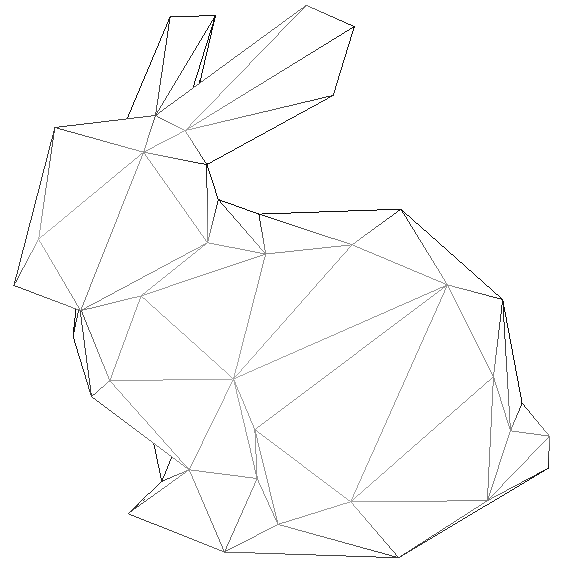
\includegraphics
		[width=0.7\columnwidth]{wireframe_40}\caption{Faces 130}\label{wireframe_40_ref}\end{subfigure}\\
	\end{tabular}
  	\caption{Wireframe versions of models in Table~\ref{tab:approx_bunny_ref}}
  	\label{tab:wireframe_ref}
  	\end{center}
	\end{table}
\end{center}

\section{Vertex Placement}

To perform the contraction of an edge $(\mathbf{v_i}, \mathbf{v_j})\rightarrow\bar{\mathbf{v}}$ we have to calcualte a new position of $\mathbf{\bar{v}}$ which is called the target. The optimal placement strategy, therefore, is to find a point for which $Q(\mathbf{\bar{v}})$ is minimal. Fortunately, since, $Q(\mathbf{\bar{v}})$ is quadratic we are guaranteed to find an unique minimizer which is a global minimum.
\begin{align}
Q(\mathbf{v}) &= \mathbf{v}^T\mathbf{A}\mathbf{v} + 2\mathbf{b}^T\mathbf{v} + c\\
\nabla Q(\mathbf{v}) &= 2\mathbf{A}\mathbf{v} + 2 \mathbf{b}
\end{align}
Solving for $\nabla Q(\mathbf{v}) = 0$, the optimal position is defined:
\begin{align}
\mathbf{\bar{v}} = -\mathbf{A}^{-1}\mathbf{b}
\end{align}
and the error:
\begin{align}
Q(\mathbf{\bar{v}}) = \mathbf{b}^T\mathbf{\bar{v}} + c = -\mathbf{b}^T\mathbf{A}^{-1}\mathbf{b} + c
\end{align}

The function used to calculate the optimal position $\mathbf{\bar{v}}$ is the following:
\begin{center}
\begin{lstlisting}[caption={LU decomposition for solving a linear system.},captionpos=b]
virtual bool optimize(Eigen::VectorXd &result) {
	Eigen::FullPivLU<Eigen::MatrixXd> lu = A.fullPivLu();
	if (!lu.isInvertible())
		return false;
	result = -lu.solve(b);
	return true;
};
\end{lstlisting}
\end{center}
Eigen::FullPivLU is LU decomposition of a matrix with complete pivoting, and related features. This decomposition provides the generic approach to solving systems of linear equations, computing the rank, invertibility, inverse, kernel, and determinant \cite{eigenLU19}.

In the case when a matrix is not invertible the following computations are performed \cite{garland99}:
\begin{enumerate}
\item If $\mathbf{A}$ is singular, find the optimal position along the line segment $(\mathbf{v_i}, \mathbf{v_j})$.
\item If this is not unique, select the better of $\mathbf{v_i}$ and $ \mathbf{v_j}$.
\end{enumerate}
In practice it is very rare that a matrix determinant is zero. Due to the limits of floating point precision. The optimal vertex placement will tend to create closely fitting approximations of the original mesh. Which at the end gives a better shaped triangles \cite{garland99}. The placement strategy for the pair of contraction $(\mathbf{v_i}, \mathbf{v_j})$ is to always move $\mathbf{v_j}$ to the position of $\mathbf{v_i}$. It eliminates a problem of storing delta of the new vertex position.

\section{Summary of Garland's Algorithm}

Below I present the complete algorithm in 5 steps. In the next chapter I will elaborate how this concept is incorporated in multithreded approach.

Algorithm \cite{garland99}:

\begin{enumerate}
\item Select a set of candidate vertex pairs $(\mathbf{v_i}, \mathbf{v_j})$.
\item Allocate a quadric $Q_i$ for each vertex $\mathbf{v_i}$.
\item For each face compute a quadric $Q_i$. Add this fundamental quadric to the vertex quadrics $Q_i, Q_k, Q_l$ and optionaly weight it appropriately.
\item For each candidate pair $(\mathbf{v_i}, \mathbf{v_j})$:
\begin{enumerate}
\item Compute $Q = Q_i + Q_j$.
\item Select a target position $\mathbf{\bar{v}}$.
\item Apply consistency checks and penalties.
\item Place pair in heap keys on cost $Q(\mathbf{\bar{v}})$
\end{enumerate}
\item Repeat unitl the desired approximation is reached:
\begin{enumerate}
\item Remove the pair $(\mathbf{v_i}, \mathbf{v_j})$ of least cost from the heap.
\item Preform contraction $(\mathbf{v_i}, \mathbf{v_j})\rightarrow\bar{\mathbf{v}}$
\item Set $Q_i = Q_i + Q_j$.
\item For each remaining pair $(\mathbf{v_i}, \mathbf{v_j})$, compute target position and cost as in step 4; update heap.
\end{enumerate}
\end{enumerate}

In the next chapter I would like to give a brief introduction to extended version of the algoritm which includes color and normals.

\chapter{Extended Simplification Algorithm}

The previous implementation includes only geometric error. In this chapter we incorporate more attributes to improve simplification. Using additionally, color and normals we can easier deceminate planar surfaces and achieve better results. However, in the noisy environment of color (which is usually the case in scans), gradient guided simplification may produce poor results.

\section{Design}
In this section we assume that each vertex is additionally associated with color $\mathbf{c} = [r \ g \ b]^T$ and $\mathbf{n} = [nx \ ny \ nz]^T$. For the sake of simplicity, lets consider an example with geometry and color only. Assume that each vertex is attributed with $\mathbf{v} = [x \ y \ z \ r \ g \ b]^T$. Figure~\ref{fig:hexagon} shows an example of such a mesh. A triangle is defined as $T = (\mathbf{p}, \mathbf{q}, \mathbf{r})$ with edges $\mathbf{h} = \mathbf{q} - \mathbf{p}$ and $\mathbf{k} = \mathbf{r} - \mathbf{p}$. Now, because our problem is more that 3 dimensional, we have to use a different method to calucalte orthogonal vectors to the plane defined by the face. Fortunately, Gram-Schmidt orthogonalization \cite{strang88} helps us to solve this problem.

\begin{figure}[H]
  \begin{center}
    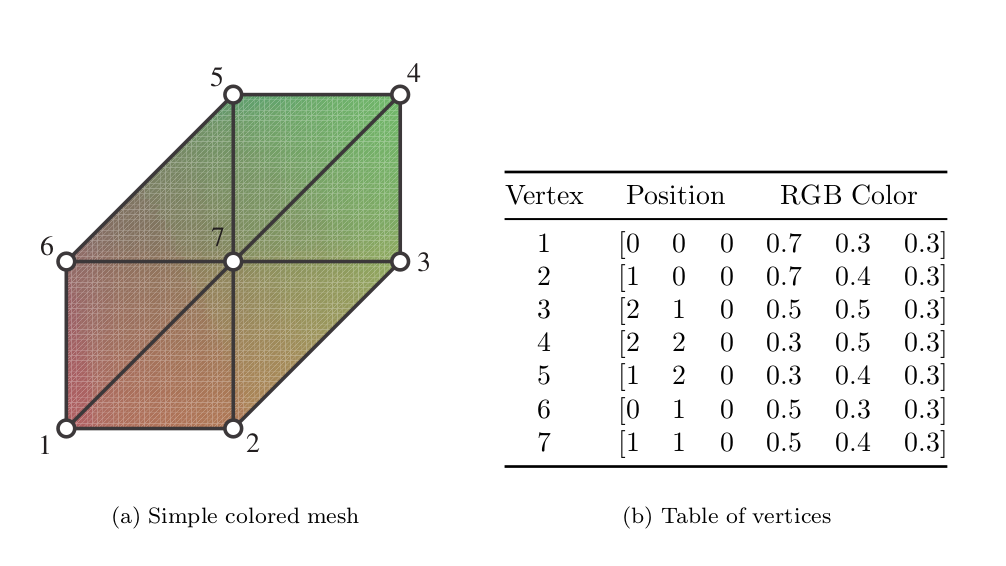
\includegraphics[width=15cm]{hexagon}
    \caption{A triangulated hexagon with color values at each vertex \cite{garland99}.}
    \label{fig:hexagon}
  \end{center}
\end{figure}

We have to find 2 vectors $\mathbf{e_1}, \mathbf{e_2}$ which are orthogonal to each other.

\begin{align}
\mathbf{e_1} &= \mathbf{h} / \norm{\mathbf{e_1}} \\
\mathbf{e_2} &= \frac{\mathbf{k} - (\mathbf{e_1} \cdot \mathbf{k})\mathbf{e_1}}{\norm{\mathbf{k} - (\mathbf{e_1} \cdot \mathbf{k})\mathbf{e_1}}}
\end{align}

Those equations give us 2 unit-length vectors which form a local coordinate system with $\mathbf{p}$ as the origin.

\begin{figure}[H]
  \begin{center}
    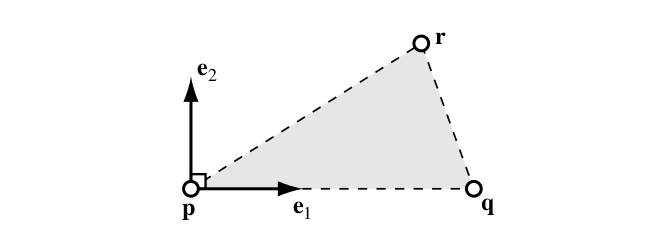
\includegraphics[width=12cm]{gram}
    \caption{Orthonomal vectors \cite{garland99}.}
    \label{fig:gram}
  \end{center}
\end{figure}

Let me define a distance from an arbitrary point $\mathbf{v}\in\mathbf{R}^n$ to the plane create by the face $T$. The quared distance of the vector $\mathbf{u} = \mathbf{p} - \mathbf{v}$ is defined as \cite{garland99}

\begin{align}
\norm{\mathbf{u}}^2 = \mathbf{u}^T\mathbf{u} = (\mathbf{u}^T\mathbf{e_1})^2 + ... +  (\mathbf{u}^T\mathbf{e_n})^2
\end{align}

We can rearrange this equation to

\begin{align}
(\mathbf{u}^T\mathbf{e_3})^2 + ... +  (\mathbf{u}^T\mathbf{e_n})^2 = \norm{\mathbf{u}}^2 - (\mathbf{u}^T\mathbf{e_1})^2 - (\mathbf{u}^T\mathbf{e_2})^2
\end{align}

The left hand side is the squared distance of $\mathbf{u}$ along all the axes perpendicular to the plane of $T$. This is a distance between this vector $\mathbf{v}$ and the plane $T$.

\begin{align}
D^2 = \mathbf{u}^T\mathbf{u} - (\mathbf{u}^T\mathbf{e_1})(\mathbf{u}^T\mathbf{e_1}) - (\mathbf{u}^T\mathbf{e_2})(\mathbf{u}^T\mathbf{e_2})
\end{align}

The quadric metric is defined then as $Q(\mathbf{v}) = \mathbf{v}^T\mathbf{A}\mathbf{v} + 2\mathbf{b}^T\mathbf{v} + c$ where

\begin{align}
\mathbf{A} &= \mathbf{I} - \mathbf{e_1}\mathbf{e_1}^T - \mathbf{e_2}\mathbf{e_2}^T\\
\mathbf{b} &= (\mathbf{p} \cdot \mathbf{e_1})\mathbf{e_1} + (\mathbf{p} \cdot \mathbf{e_2})\mathbf{e_2} - \mathbf{p}\\ 
\mathbf{c} &= \mathbf{p} \cdot \mathbf{p} - (\mathbf{p} \cdot \mathbf{e_1})^2 - (\mathbf{p} \cdot \mathbf{e_2})^2 
\end{align}

The matrix A from \ref{fig:hexagon} is then

\begin{align}
\left[
\begin{array}{rrrrrr}
0.06 & 0 & 0 & 0 & -0.59 & 0\\
0 & 0.23 & 0 & 1.15 & 0 & 0\\
0 & 0 & 6.00 & 0 & 0 & 0\\
0 & 1.15 & 0 & 5.77 & 0 & 0\\
-0.59 & 0 & 0 & 0 & 5.94 & 0\\
0 & 0 & 0 & 0 & 0 & 6.00
\end{array}\right]
\end{align}

Building the quadric and finding the optimal position is exactly the same like in the geometry only case. To use different metric we have to only change computations of orthagonal vectors. In Table\ref{tab:color_simplification} we can see the results of using color and geometry metric error. We can easily notice that the simplifcation follows the color pattern. In some cases its a desired features, however, we have to be carefule about the noise of the gradient.

\begin{center}
  	\begin{table}[H]
  	\begin{center}
  	\begin{tabular}{cc}
	\begin{subfigure}{0.5\textwidth}\centering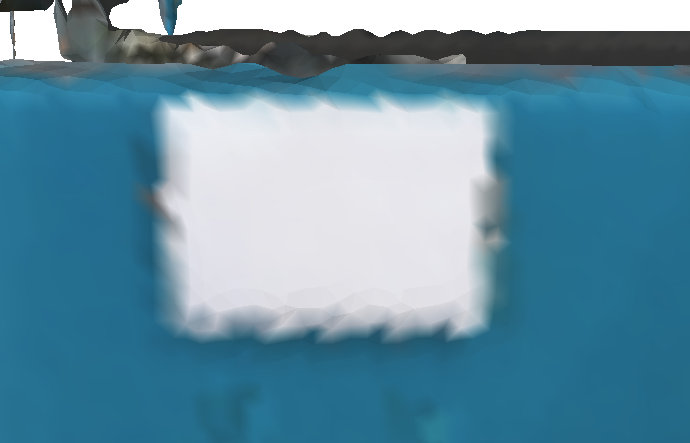
\includegraphics
		[width=1\columnwidth]{color_1}\caption{Original}\label{color1}\end{subfigure}&	
	\begin{subfigure}{0.5\textwidth}\centering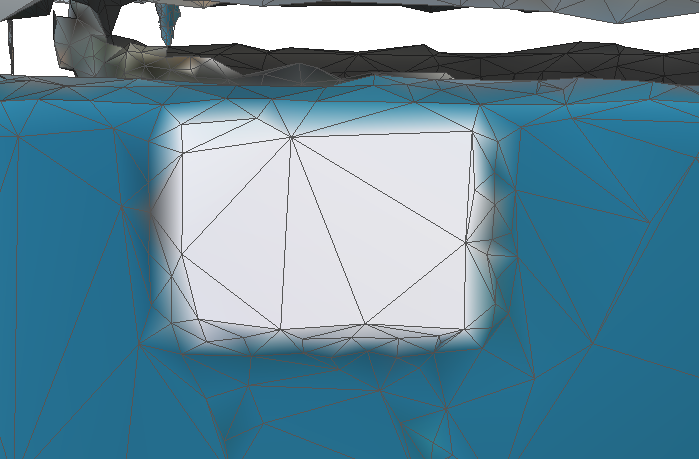
\includegraphics
		[width=1\columnwidth]{color_2}\caption{Color and geometry simplification}\label{color2}\end{subfigure}\\
		\newline
			\begin{subfigure}{0.5\textwidth}\centering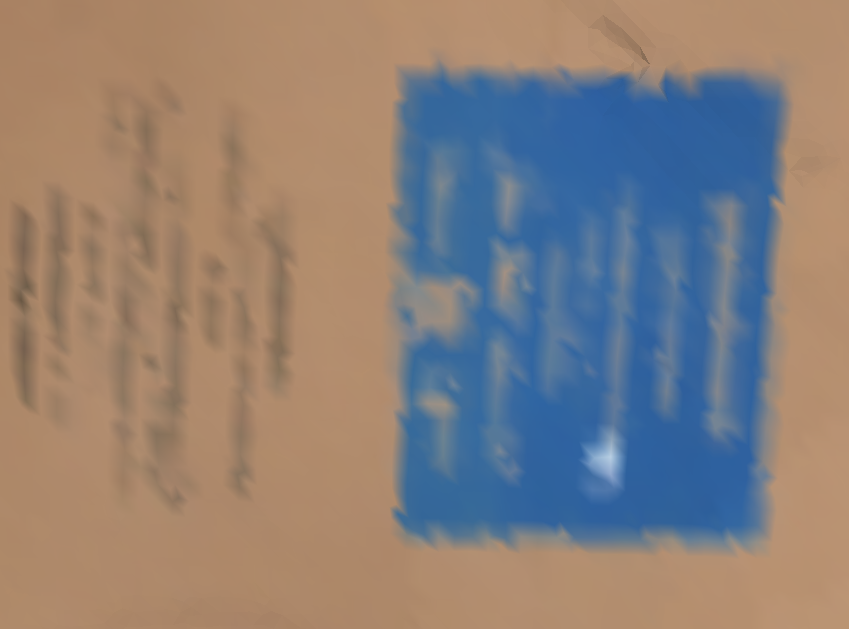
\includegraphics
		[width=1\columnwidth]{color_4}\caption{Original}\label{color1}\end{subfigure}&	
	\begin{subfigure}{0.5\textwidth}\centering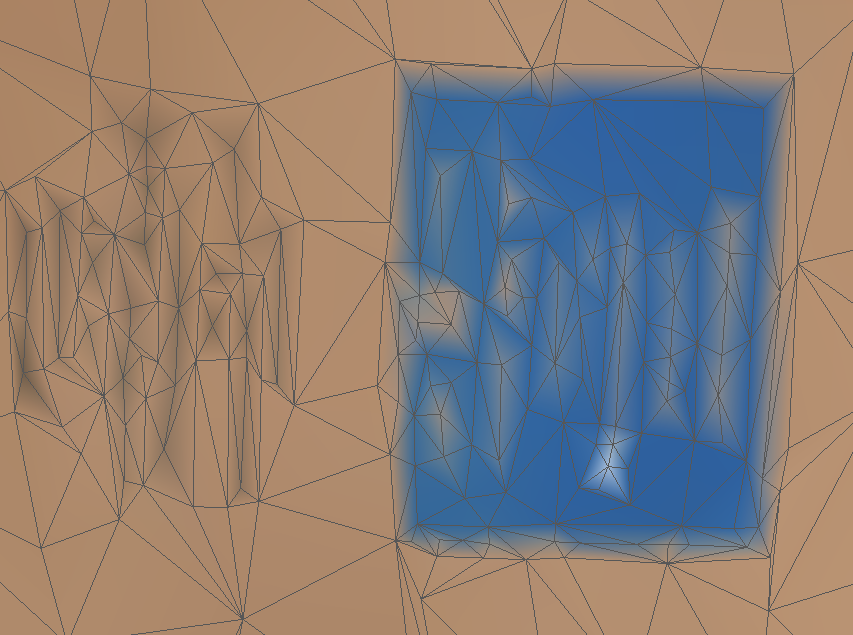
\includegraphics
		[width=1\columnwidth]{color_3}\caption{Color and geometry simplification}\label{color2}\end{subfigure}
		\end{tabular}
  	\caption{Comparison of gradient guided simplification.} \label{tab:color_simplification}
  	\end{center}
	\end{table}
\end{center}


\chapter{Parallel Implementation of the Algorithm}

In this chapter, I will describe my approach to design a parallel version of Garland's simplification algorithm. First, I would like to describe Producer-Consumer design patter, libraries and ideas used in the implementation to make it thread-safe. Next, I will analize the speedup and potential problems which can arose during an exacution. Finally, summarize the approach and elaborate further improvements.

\section{Producer Consumer}



%\include{StateOfTheArt}
%\include{Problem}
%\include{HowTo}
%\include{Results}
%  Conclusions (Zusammenfassung):
\chapter{Zusammenfassung}
\thispagestyle{empty}% no page number in chapter title page
Am Schlu� werden noch einmal alle wesentlichen Ergebnisse
zusammengefa�t.  Hier k�nnen auch gemachte Erfahrungen beschrieben
werden.  Am Ende der Zusammenfassung kann auch ein Ausblick folgen,
der die zuk�nftige Entwicklung der behandelten Thematik aus der Sicht
des Autors darstellt.

% Appendix (Anh�nge), could have multiple chaper-files:
\appendix
\chapter{Examples of simplification}
\thispagestyle{empty}% no page number in chapter title page

The examples below present the simplification of a mesh generated from a dense point cloud scanned in the NavVis office. The mesh has 507277 vertices and 973168 faces.

\begin{sidewaysfigure}[ht]
    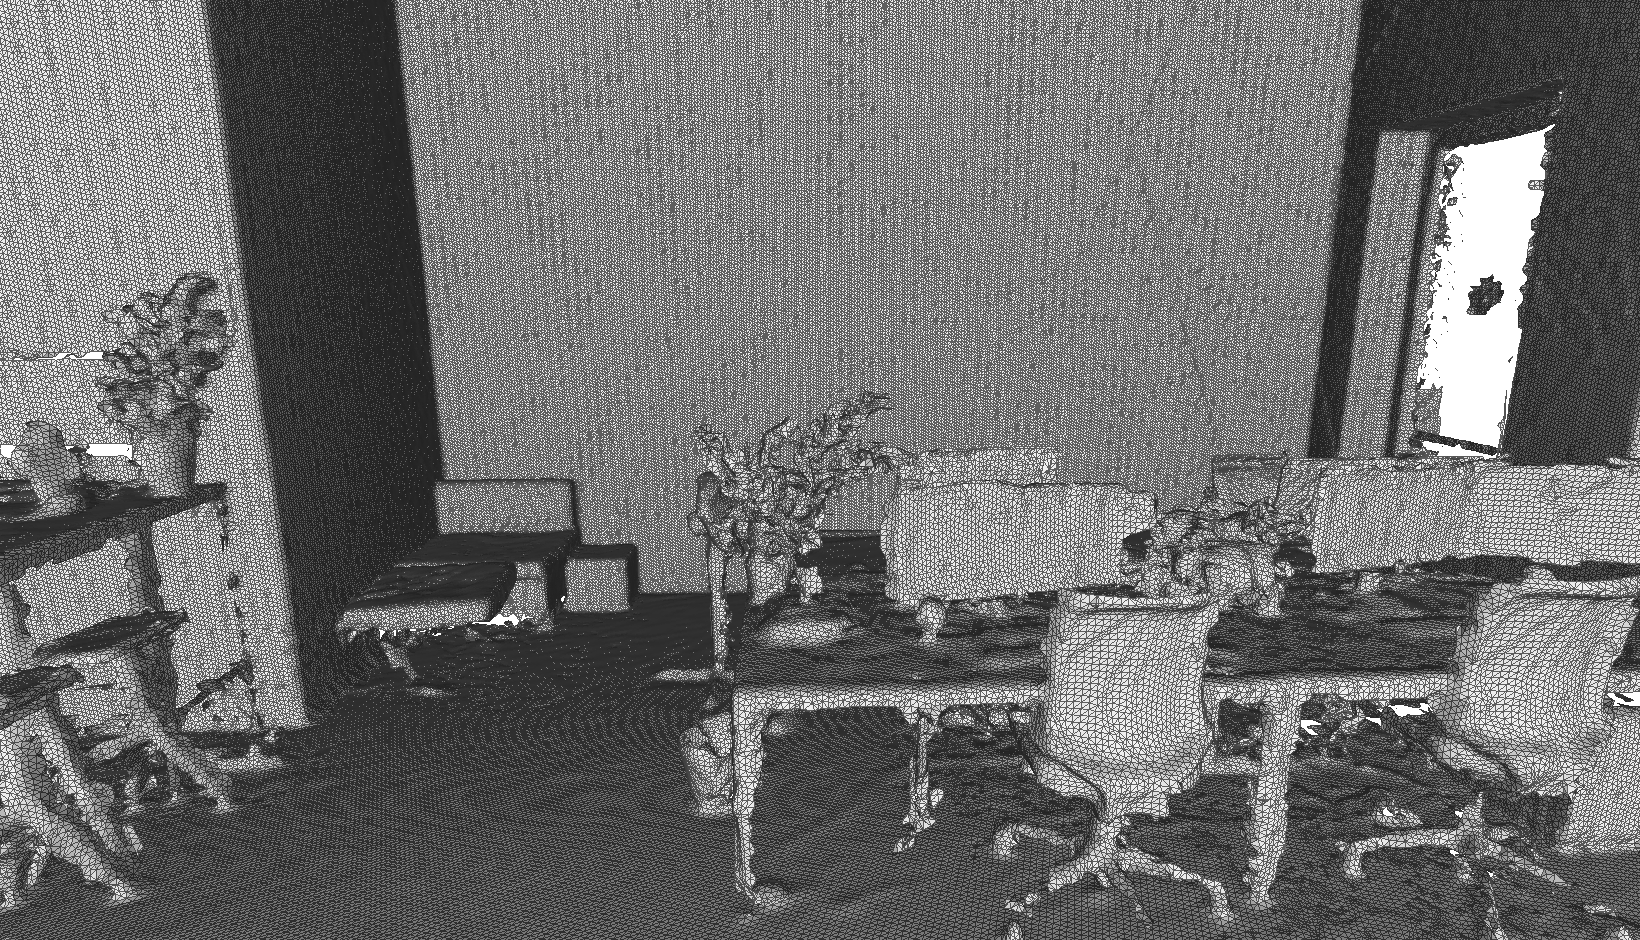
\includegraphics[width=20cm]{final_0}
    \caption{Original mesh with evenly distributed triangles.}
    \label{fig:final_0}
\end{sidewaysfigure}

\newpage
\begin{sidewaysfigure}[ht]
    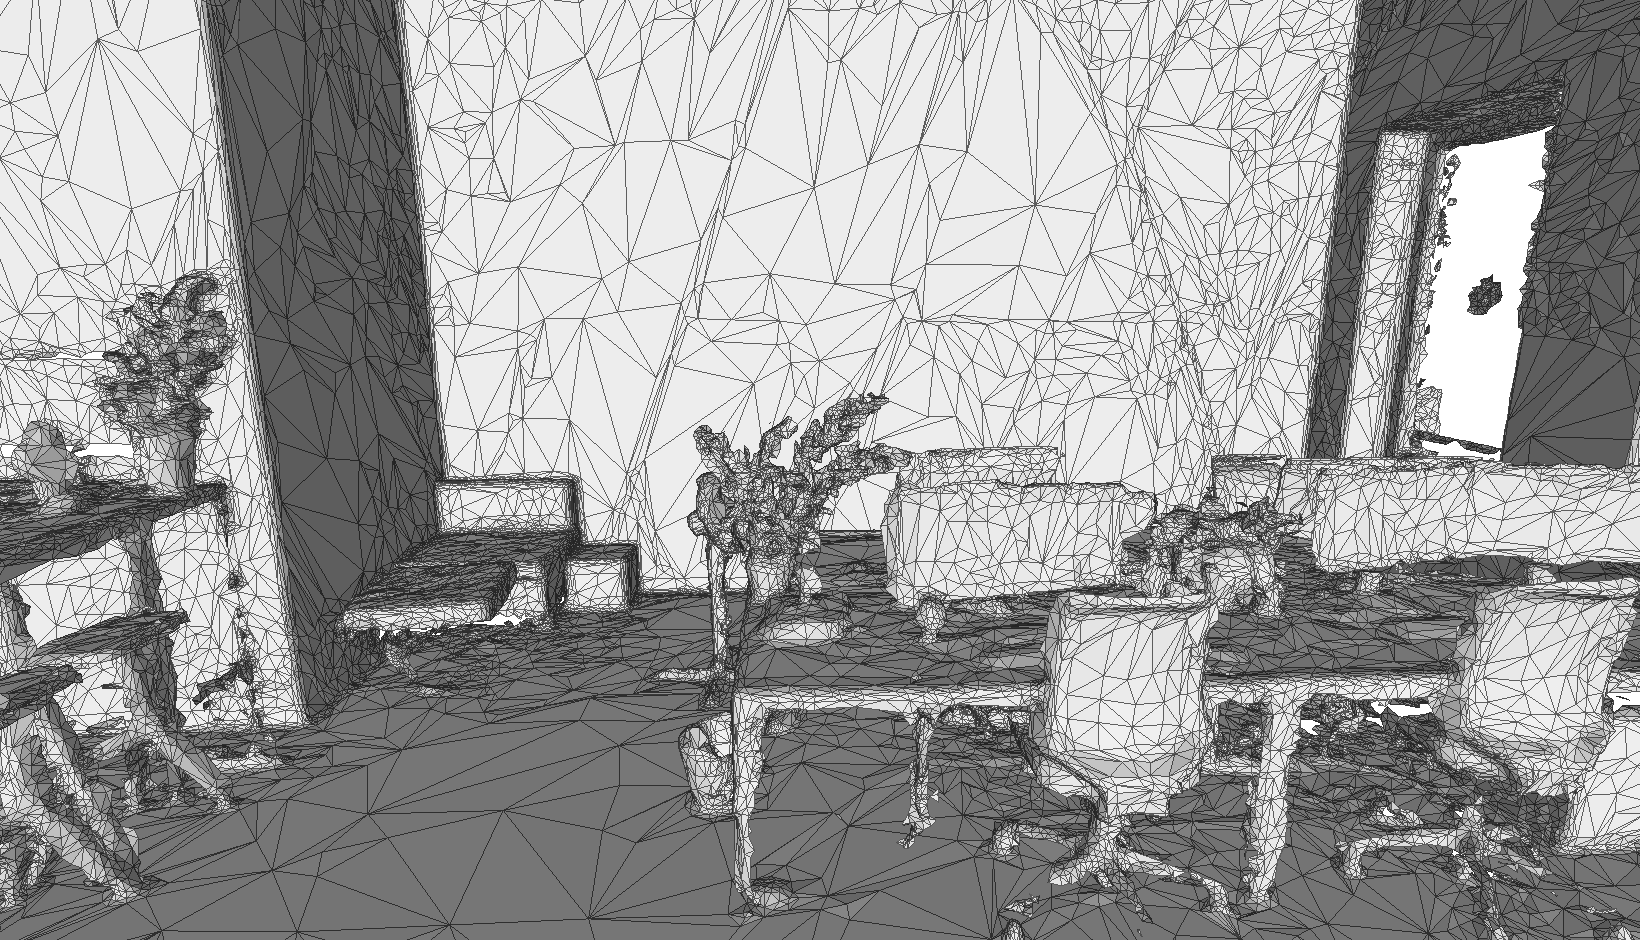
\includegraphics[width=20cm]{final_3}
    \caption{Simplified mesh to 15\% of the original using [geometry]}
    \label{fig:final_3}
\end{sidewaysfigure}

\newpage
\begin{sidewaysfigure}[ht]
    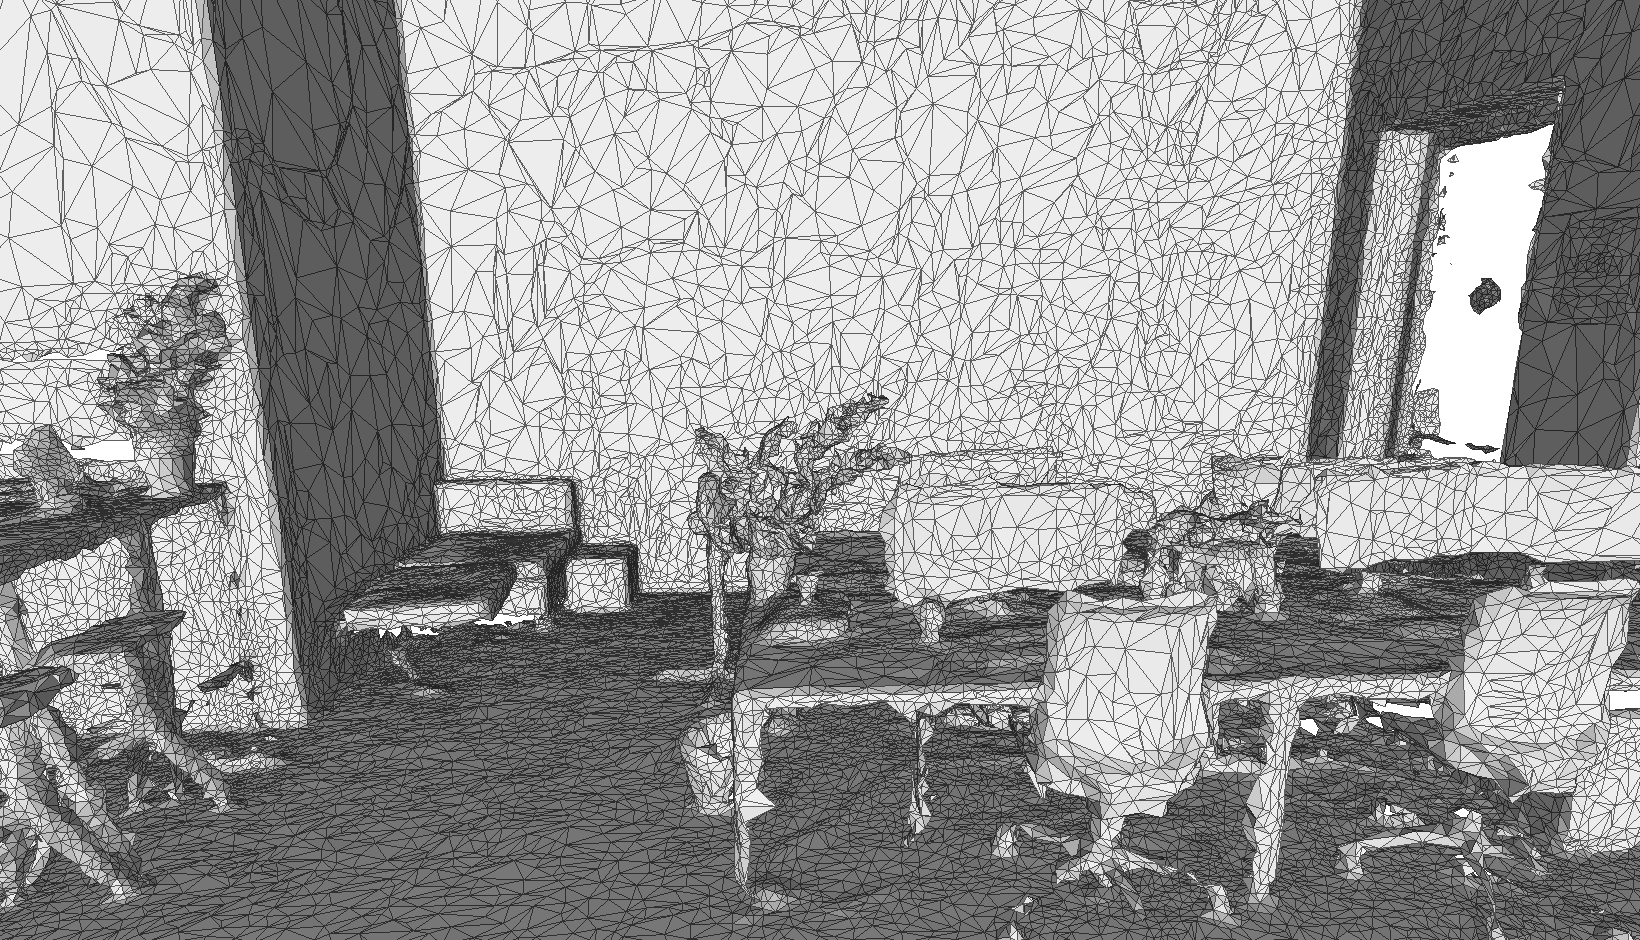
\includegraphics[width=20cm]{final_6}
    \caption{Simplified mesh to 15\% of the original using [geometry, color]}
    \label{fig:final_6}
\end{sidewaysfigure}

\newpage
\begin{sidewaysfigure}[ht]
    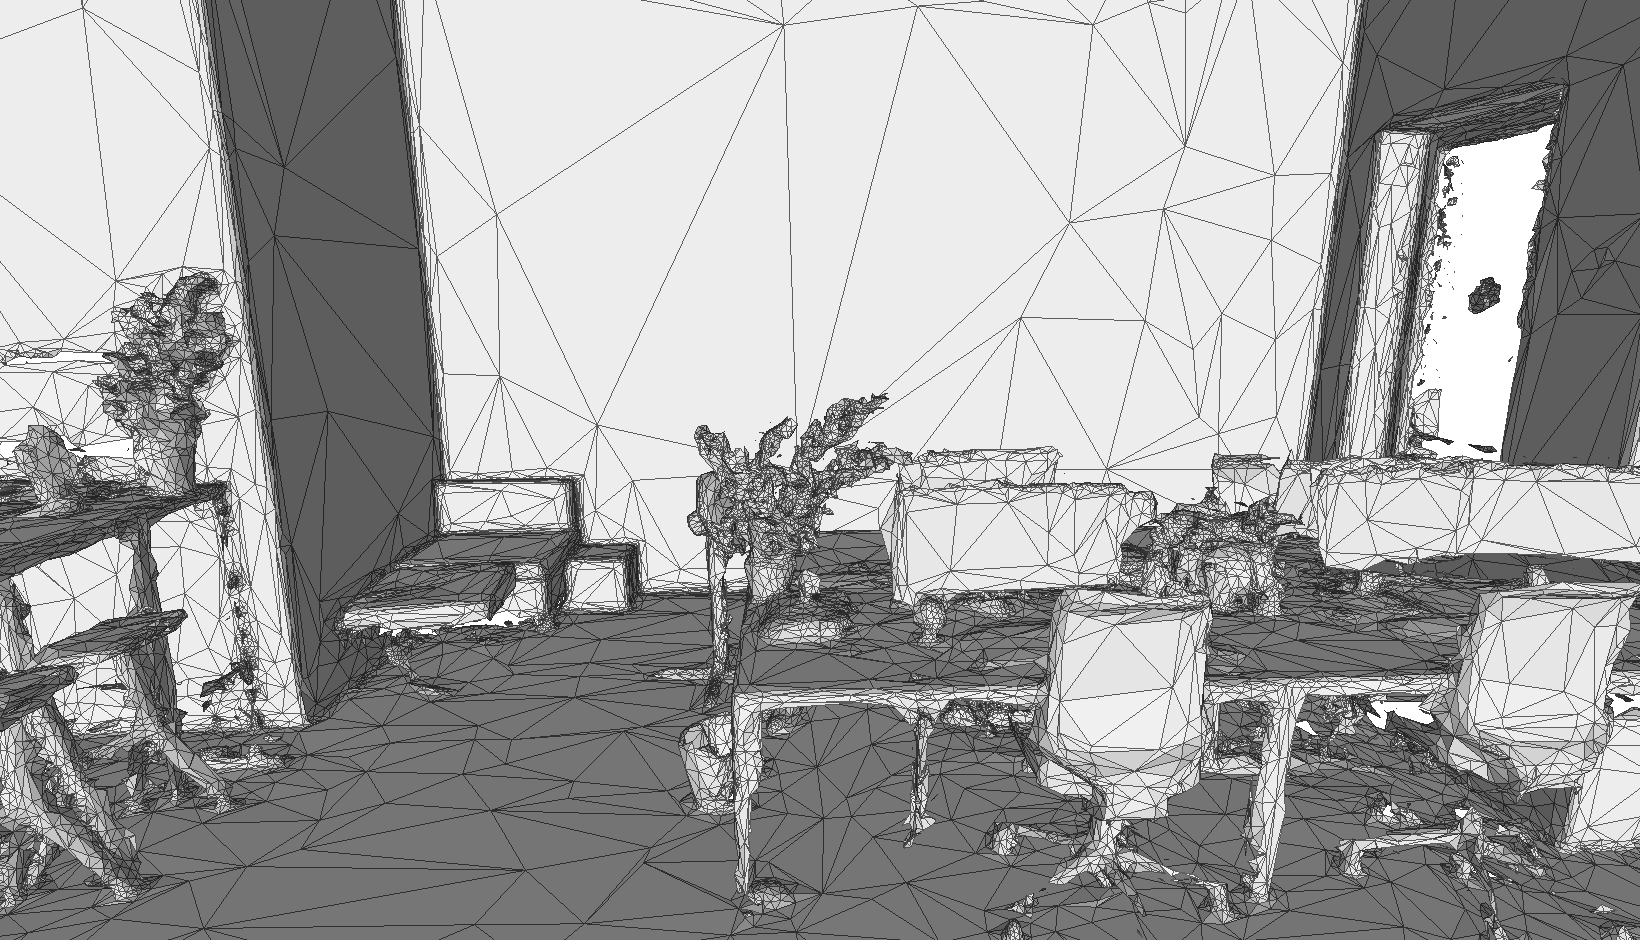
\includegraphics[width=20cm]{final_9}
    \caption{Simplified mesh to 15\% of the original using [geometry, color, normal]}
    \label{fig:final_9}
\end{sidewaysfigure}
% List of figures (Abbildungsverzeichnis):
\listoffigures
% List of tables (Tabellenverzeichnis):
\listoftables
% Glossary (Glossar):
%\include{Glossary}
% List of formulae (Liste der Formelzeichen):
%\include{Formulae}
% Abbreviations (Abk�rzungsverzeichnis):
%\include{Abbreviations}

% References (Literaturverzeichnis):
% a) Style (with numbers: use unsrt):
\bibliographystyle{alpha}
% b) The File:
\bibliography{Bibliography}

\end{document} %*****************************************************
